\section{Аналитический раздел}
\subsection{Постановка задачи}
В соответствии с заданием на курсовую работу по дисциплине <<Операционные системы>> требуется разработать ПО, позволяющее задавать определённые действия системы движением нескольких пальцев по тачпаду.

Для выполнения задания требуется решить следующие задачи:
\begin{enumerate}
	\item провести анализ существующих подходов к обработке устройств ввода;
	\item провести анализ существующих способов задания действий движением нескольких пальцев по тачпаду;
	\item провести анализ возможности исполнения системой заданных действий;
	\item разработать алгоритмы, необходимые для реализации ПО;
	\item разработать ПО, предоставляющее требуемую функциональность;
	\item провести исследование разработанного ПО.
\end{enumerate}

Для разработки и тестирования данной работы используется портативный компьютер \texttt{Huawei Matebook X Pro} и операционная система \texttt{Linux} с дистрибутивом \texttt{Kali Linux}.

\subsection{Загружаемый модуль ядра}

Ядро Linux относится к классу монолитных. В архитектуре данного класса прикладные приложения выполняются посредством создания отдельной ветки кода в пространстве ядра. Поскольку в ранних версиях расширение функциональности требовало перекомпиляции ядра, что было недопустимо для систем промышленного уровня, позднее была добавлена технология модуля ядра. Модуль ядра может реализовывать драйвер устройства, файловую систему или сетевой протокол

К преимуществам такого подхода следует отнести сокращение неиспользуемого кода в базовом ядре и, как следствие, уменьшение занимаемой памяти. Недостатком является фрагментация ядра, после загрузки
модулей, несмотря на то, что код базового ядра не фрагментируем. Фрагментация ведет к незначительному снижению производительности из-за
увеличения пропусков записей TLB. Также использование загружаемого модуля снижает безопасность системы, поскольку злоумышленники, имея
доступ в пространство ядра, могут скрывать процессы и файлы.

\subsubsection{Компоненты модуля ядра}

Загрузка модуля осуществляется с помощью команд \texttt{insmod} или \texttt{modprobe}. Отличие заключается в том, что \texttt{modprobe} разрешает зависимости модулей. При загрузке вызывается функция входа, определенная в модуле. Для указания ее назначения используется макрос \texttt{module\_init}. При корректной загрузке функция входа возвращает 0. В ином случае, модуль не будет загружен.

Для просмотра списка загруженных модулей и информации об отдельном модуле используются команды \texttt{lsmod} и \texttt{modinfo} соответственно. Командой \texttt{rmmod} осуществляется выгрузка модуля, при которой вызывается функция выхода. Для неё используется макрос \texttt{module\_exit}.

\subsubsection{Драйвера}

Одной из разновидностей модуля ядра являются драйверы устройств. Драйверы полностью скрывают детали, касающиеся работы устройства и предоставляют чёткий программный интерфейс для работы с аппаратурой. В Linux драйверы устройств бывают трёх типов:

\begin{enumerate}
	\item драйверы первого типа являются частью программного кода ядра. Соответствующие устройства автоматически обнаруживаются системой и
	становятся доступны доя приложений;
	
	\item драйверы второго типа представлены загружаемыми модулями ядра. Они	оформлены в виде отдельных файлов. Для их подключения необходимо выполнить команду подключения модуля. Если необходимости в
	использовании нет, модуль можно выгрузить из памяти. Использование
	модулей обеспечивает большую гибкость, так как каждый драйвер может быть переконфигурирован без остановки системы;
	
	\item в драйверах третьего типа программный код драйвера поделён между ядром и специальной утилитой, предназначенной для управления данным устройством.
\end{enumerate}

Во всех драйверах взаимодействие с устройством осуществляет ядро или
модуль ядра, а пользовательские программы взаимодействуют через специальные файлы, расположенные в каталоге \texttt{/dev} и его подкаталогах.

\subsubsection{Драйвер устройства ввода}

Драйвер устройства ввода -- это модуль, обеспечивающий возможность взаимодействия с интерактивным устройством через события.

Алгоритм регистрации драйвера устройства ввода \cite{docs}: 
\begin{enumerate}
	\item заполнение структуры \texttt{struct input\_handler};
	\item регистрация обработчика функцией \texttt{input\_register\_handler}. 
\end{enumerate}

Для обработки устройств ввода можно воспользоваться подсистемой ввода/вывода. Данная подсистема выполняет запросы файловой подсистемы и подсистемы управления процессами для доступа к периферийным устройствам (дискам, магнитным лентам, терминалам и т.д.). Она обеспечивает необходимую буферизацию данных и взаимодействует с драйверами устройств -- специальными модулями ядра, непосредственно обслуживающими внешние устройства.

\subsection{Передача информации из пространства ядра в пространство пользователя}

Файловая система (ФС) \texttt{proc} создана для того, чтобы в режиме пользователя получать информацию о процессах и ресурсах, которые используют эти процессы. ФС \texttt{proc} формирует интерфейс, позволяющий обращаться к структурам ядра.

В ФС \texttt{proc} можно создавать свои файлы, ссылки, директории. Для этого в ядре предоставляется структура \texttt{proc\_dir\_entry}, определенная в файле \texttt{<fs/proc/internal.h>}. Для определения обратных вызовов чтения и записи предоставляется структура \texttt{proc\_ops}. Данная структура определена в файле
\texttt{<include/linux/proc\_fs.h>}, наиболее важные поля которой представлены в листинге \ref{lst:procops}.

\begin{lstlisting}[label=lst:procops,caption=Структура proc\_ops, language=c]
struct proc_ops {
	unsigned int proc_flags;
	int	(*proc_open)(struct inode *, struct file *);
	ssize_t	(*proc_read)(struct file *, char __user *, size_t, loff_t *);
	...
	ssize_t	(*proc_write)(struct file *, const char __user *, size_t, loff_t *);
	...
	int	(*proc_release)(struct inode *, struct file *);
	...
} __randomize_layout;
\end{lstlisting}

Использование функций \texttt{proc\_create} и \texttt{remove\_proc\_entry}, определённых в файле \texttt{<include/linux/proc\_fs.h>}, позволяет регистрировать и отменять регистрацию файла в \texttt{proc}. Для взаимодействия ядра с приложениями используется функция \texttt{copy\_to\_user}, определение которой представлено в файле \texttt{<include/linux/uaccess.h>}. Данная функция копирует блоки данных из ядра в пространство пользователя. Для передачи информации в пространство ядра используется функция \texttt{copy\_from\_user}.

\subsection{Прерывания}

Прерывания делятся на:
\begin{itemize}
	\item исключения (деление на ноль, переполнение стека), синхронные;
	\item системные вызовы (программные) - вызываются с помощью соответствующей команды из программы (\texttt{int 21h}), синхронные;
	\item аппаратные прерывания (прерывания от системного таймера, клавиатуры), асинхронные. 
\end{itemize}

Прерывания делятся на 2 группы:

\begin{itemize}
	\item быстрые;
	\item медленные. 
\end{itemize}

Для того чтобы сократить время обработки медленных прерываний, они делятся на 2 части:

\begin{itemize}
	\item \texttt{top half}, верхняя половина, запускается в результате получения процессором сигнала прерывания;
	\item \texttt{bottom half}, нижняя половина, отложенные вызовы.
\end{itemize}

Существует несколько способов реализации “нижней половины“
обработчика: 
\begin{itemize}
	\item \texttt{softirq};
	\item тасклет (\texttt{tasklet});
	\item очереди работ (\texttt{workqueue}).
\end{itemize}
\subsubsection{Обработчики аппаратных прерываний}

Обработчик прерывания должен выполнять минимальный объем действий и завершаться как можно быстрее. Обычно такой обработчик прерывания сохраняет данные, поступившие от внешнего устройства, в буфере ядра. 
Но для того чтобы обработать прерывания полностью, обработчик аппаратного прерывания должен инициализировать постановку в очередь на выполнение отложенное действие.

\subsubsection{Очереди работ}

Очереди работ являются обобщённым механизмом отложенного выполнения, в котором функция обработчика, реализующая соответствующие действия, может блокироваться.

\texttt{struct workqueue\_struct} - описывает очередь работ.

\begin{lstlisting}[language=c, label=some-code, caption=Структура workqueue\_struct]
	struct workqueue_struct {
		struct list_head pwqs; /* WR: all pwqs of this wq */
		struct list_head list; /* PR: list of all workqueues */
		...
		struct pool_workqueue  *dfl_pwq; /* PW: only for unbound wqs */
		...
		struct pool_workqueue __percpu *cpu_pwqs; /* I: per-cpu pwqs */
		...
	};
\end{lstlisting}

\texttt{struct work\_struct} - описывает работу (обработчик нижней половины).

\begin{lstlisting}[language=c, label=some-code, caption=Структура workqueue\_struct]
	struct work_struct {
		atomic_long_t data;
		struct list_head entry;
		work_func_t func;
		...
	};
\end{lstlisting}

Работа может инициализироваться 2-мя способами:

\begin{itemize}
	\item статически;
	\item динамически.
\end{itemize}

При статической инициализации используется макрос:

\begin{lstlisting}[language=c, label=some-code, caption=статическая инициализация]
	DECLARE_WORK(name, void (*func)(void *));
\end{lstlisting}

где: \texttt{name} -- имя структуры \texttt{work\_struct}, \texttt{func} -- функция, которая вызывается из \texttt{workqueue} -- обработчик нижней половины.

При динамической инициализации используются макросы:

\begin{lstlisting}[language=c, label=some-code, caption=динамическая инициализация]
	INIT_WORK(sruct work_struct *work, void (*func)(void),void *data);
\end{lstlisting}

После того, как будет инициализирована структура для объекта \texttt{work}, следующим шагом будет помещение этой структуры в очередь работ. Это можно сделать несколькими способами. Во-первых, можно добавить работу (объект \texttt{work}) в очередь работ с помощью функции \texttt{queue\_work} (которая назначает работу текущему процессору). Во-вторых, можно с помощью функции \texttt{queue\_work\_on} указать процессор, на котором будет выполняться обработчик.

\subsection{Поток ядра}

Потоки или нити ядра работают внутри пространства ядра и не имеют своего собственного адресного пространства. Они могут независимо назначаться на выполнение. Потоки используют стандартные механизмы синхронизации ядра, такие как \texttt{sleep} или \texttt{wakeup}.

Потоки ядра используются для выполнения асинхронного ввода-вывода. Ядро создаёт поток для обработки запросов каждой такой операции. Потоки также могут быть использованы для обработки прерываний.

\subsubsection{Переключение потоков}

Переключение потоков является основной задачей планировщика. В ОС Linux механизм планирования основывается на приоритетах. Когда процесс просыпается, ядро устанавливает значение текущего приоритета, равное значению приоритета сна события или ресурса, на котором он был заблокирован. Такой процесс будет назначен на выполнение раньше, чем другие процессы в режиме задачи.

Когда процесс завершил выполнение системного вызова и находится в состоянии возврата в режим задачи, его приоритет сбрасывается обратно в значение текущего приоритета в режиме задачи.

\subsection{Запуск процессов пользователя из пространства ядра}

Использование функции \texttt{call\_usermodhelper} \cite{src} позволяет выполнять процесс пользователя из процесса ядра. Работа этой функции аналогична работе вызова \texttt{exec()} в пространстве пользователя. Особенность данного метода заключается в том, что процесс запускается без управляющего терминала и с нестандартным окружением. Внутренняя реализация функции представлена на рисунке \ref{fig:umh}.

\clearpage

\begin{figure}[h!btp]
	\centering
	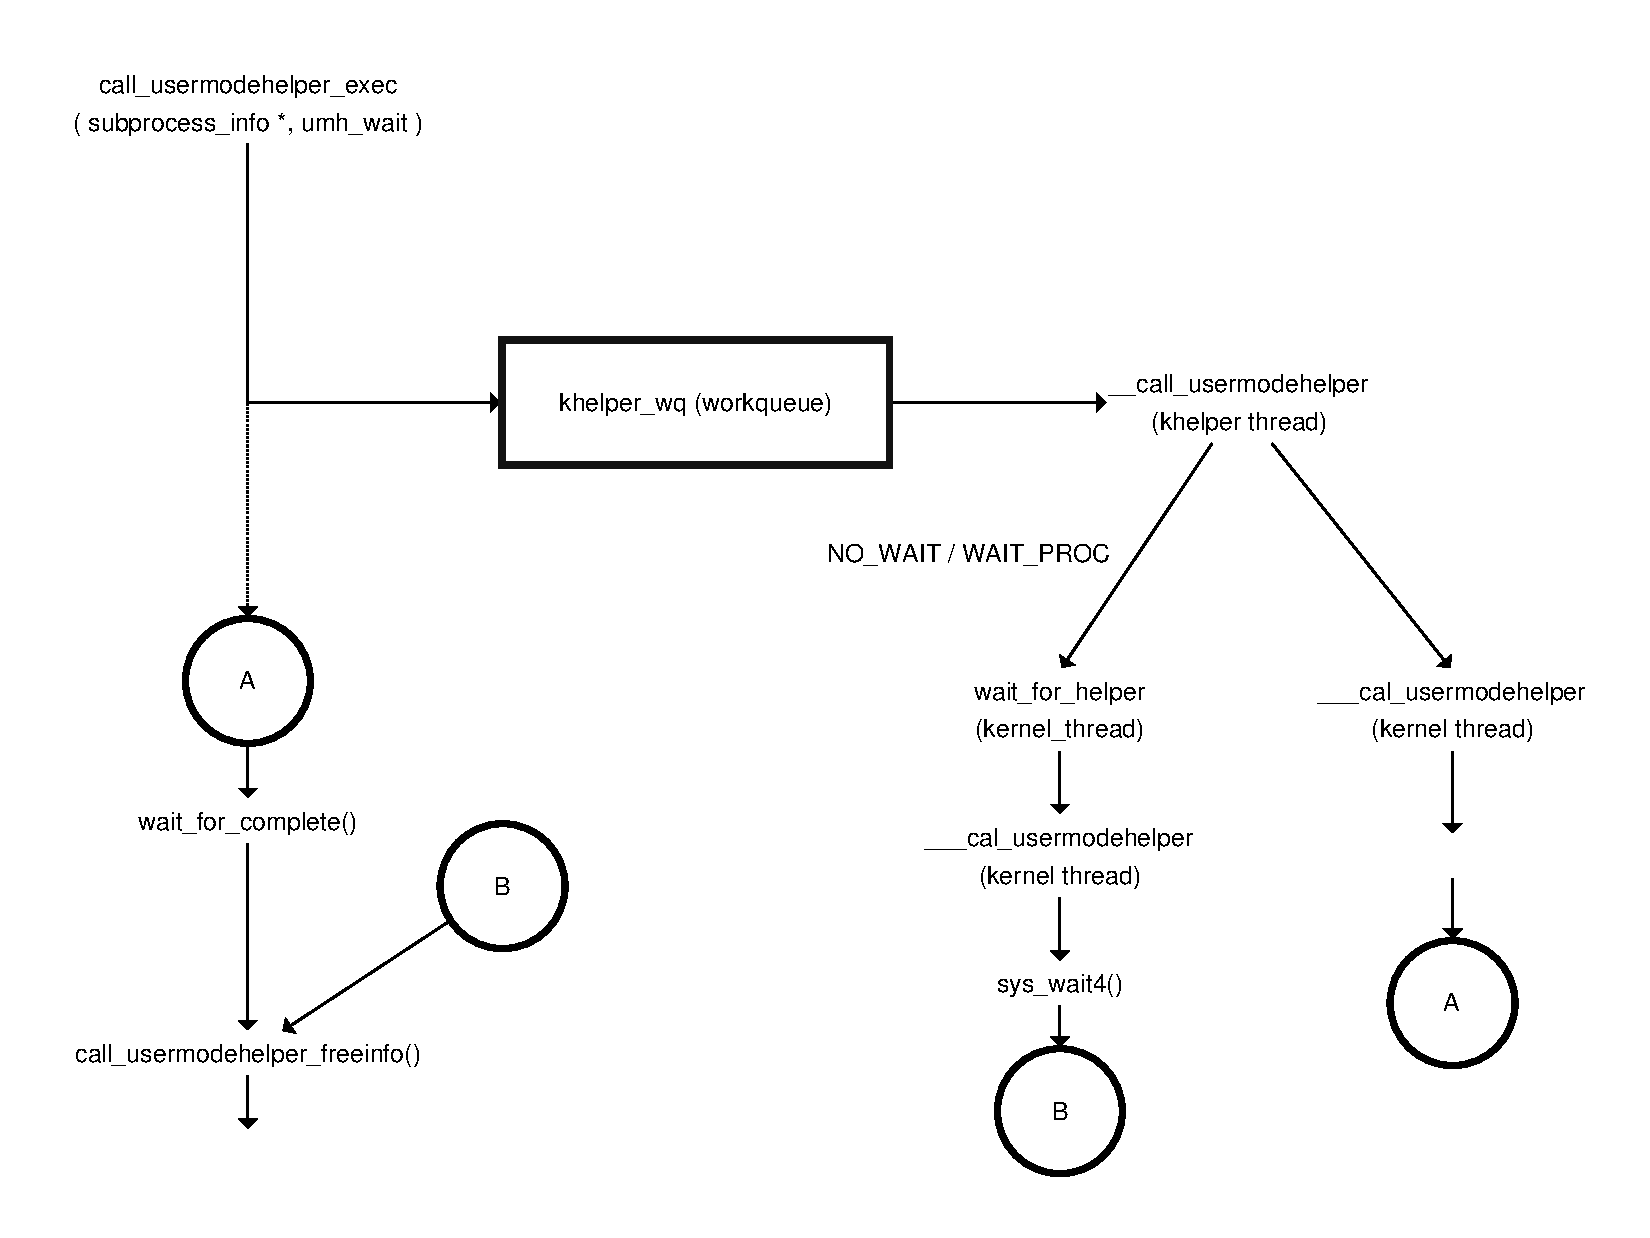
\includegraphics[width=0.9\textwidth]{inc/usermodehelper.pdf}
	\caption{Внутренняя реализация функции \texttt{call\_usermodehelper}}
	\label{fig:umh}	
\end{figure}

\subsection{Определение нескольких пальцев на тачпаде}

Для определения нескольких пальцев на тачпаде можно воспользоваться \texttt{Multi Touch} протоколом. Для каждого пальца отправляется набор событий, содержащий: 

\begin{itemize}
	\item \texttt{ABS\_MT\_SLOT} -- порядковый номер;
	\item \texttt{ABS\_MT\_TRACKING\_ID} -- идентификатор;
	\item \texttt{ABS\_MT\_POSITION\_X} -- координата X;
	\item \texttt{ABS\_MT\_POSITION\_Y} -- координата Y.
\end{itemize}

Каждый набор событий завершается событием \texttt{SYN\_REPORT}. 

При удалении пальца с тачпада идентификатор \texttt{ABS\_MT\_TRACKING\_ID} для соответствующего пальца будет равен -1. Пример потока событий для двух пальцев показан в листинге \ref{lst:mt2}.

\clearpage

\begin{lstlisting}[language=c, label=lst:mt2, caption={Поток событий для двух пальцев}]
	ABS_MT_SLOT 0
	ABS_MT_TRACKING_ID 45
	ABS_MT_POSITION_X x[0]
	ABS_MT_POSITION_Y y[0]
	ABS_MT_SLOT 1
	ABS_MT_TRACKING_ID 46
	ABS_MT_POSITION_X x[1]
	ABS_MT_POSITION_Y y[1]
	SYN_REPORT
\end{lstlisting}

\subsection{Выводы}

В результате проведённого анализа было решено:
\begin{enumerate}
	\item для выполнения задания разработать драйвер устройства ввода, который должен быть реализован как загружаемый модуль ядра;
	\item для выполнения заданных действий использовать очередь работ;
	\item для задания действий системы воспользоваться скриптовым языком \texttt{bash};
	\item для передачи инструкций в драйвер использовать виртуальную систему \texttt{/proc/}.
\end{enumerate}

\clearpage